% !TeX root = ../main.tex
% Add the above to each chapter to make compiling the PDF easier in some editors.

%TODO: Context sensitive syntax for this analysis!!! and improving vov analysis!!!

\chapter{Combatting Precision Loss}\label{chapter:mainContributions}
  In this chapter we will describe our approach to reduce the precision loss described in \autoref{section:precisionLoss}. We will first use the syntax for flow sensitive analyses from \autoref{chapter:background} to formally define the idea. After that we explain the concrete implementation of the approach into the \gob\ analyzer.
  \section{Formal description}
    %TODO: SOME TEXT!!!
    \subsection{Taint analysis}\label{section:formalTaint}
      The basic idea to combat the precision loss is to track for each procedure which variables have been written or have possibly been altered in some other way. This information is then used in the values-of-variables analysis when combining the abstract state from the caller with the abstract return state given by the callee at the end of the procedure.\\
      In the following we will call a variable that has been written or altered in the current procedure context "tainted". Therefore, we introduce a new taint analysis tracking which variables have been tainted within the context of the current procedure. It is worth mentioning that our notion of taintedness is related but different from other uses of this concept.\\
      \\
      Let us now formulate the syntax for our taint analysis: Since we want to find a collection of tainted variables per program point, a suitable domain for this analysis is the powerset of the set of variables $X$ ordered by the subset relation:
      \[\mathbb{D}_\textsf{t} = 2^X \text{ with } \sqsubseteq_\textsf{t} = \subseteq\]
      To be compatible with the notion of partially context sensitive analyses from \autoref{section:partialCtxSens} we need to also specify a context domain $\mathbb{C}_\textsf{t}$ which we will define later.
      From that follows that we seek to compute a mapping from program points (with context) to sets of variables, i.e., $\eta_\textsf{t}: (N \times \mathbb{C}_\textsf{t}) \rightarrow \mathbb{D}_\textsf{t}$. To interpret this with the goal of our taint analysis in mind, we note that $\eta_\textsf{t} [n, \bullet] = T$ will denote that $T$ is the set of possibly tainted variables at program point $n$. Expressed differently this means that for any variable $x \in T$ we cannot exclude that this variable was altered between the start of the procedure $n$ is in up until the program point $n$.\\
      It remains to define $\mathbb{C}_\textsf{t}$, $\textsf{init}^{\#}_\textsf{t}$, $\textsf{enter}^{\#}_\textsf{t}$ and $\textsf{combine}^{\#}_\textsf{t}$ as well as the abstract effects of actions $[\![ A ]\!]^{\#}$. Recall that the notion of a "tainted" variable is defined in relation to the current procedure. This means we want to start fresh whenever we enter a procedure and start without any variable being initially tainted. It is worth pointing out that the entry to a procedure call does not depend on the state where it is called. Therefore, we design our analysis to be context-insensitive, i.e., \[\mathbb{C}_\textsf{t} = \{\bullet\} \text{ and trivially } \textsf{context}^{\#}_\textsf{t}\ T = \bullet\]\\
      With these considerations we define $textsf{enter}^{\#}_\textsf{t}$ and $\textsf{init}^{\#}_\textsf{t}$ as follows:
      \[\textsf{enter}^{\#}_\textsf{t}\ T = \textsf{init}^{\#}_\textsf{t} = \emptyset\]
      It is worth pointing out here that the function $\textsf{enter}^{\#}_\textsf{t}\ T$ is always equal to the empty set irregardless of its argument $T$. Therefore, it computes the same function context for each call of a certain procedure making our taint analysis inherently context insensitive.\\
      When combining the caller state with the returned callee state, we note that anything that we need to keep the tainted set from before the call, as a tainted variable can get never get "untainted" again, no matter what the procedure does. In addition to that we will add the set returned by the callee, as anything tainted in the call needs to be considered tainted in the caller as well. This is because we want to know which variables have been altered in a procedure call, no matter if the tainting happened within the procedure itself or within a procedure called by the procedure. This leaves us with the following equation for the $\textsf{combine}^{\#}_\textsf{t}$ function:
      \[ \textsf{combine}^{\#}_\textsf{t}\ (T_\textsf{cr}, T_\textsf{ce}) = T_\textsf{cr} \cup (T_\textsf{ce} \backslash Locals_\textsf{ce}) \]
      Note that we removed the callee local variables $Locals_\textsf{ce}$ because these are not accessible by the caller and all of its callers anyway, so it is not useful to keep track of them.\\
      Lastly we define the abstract effects of actions. Most of these (including checks) do not do anything besides propagating through the state from before. The only major exception is a variable assignment. For these we note that this specific variable, which the value is assigned to is added to the tainted set. This is independent of the expression that evaluates to the assigned value, as we are only interested in the fact that the variable on the left of the assignment is altered. This leaves us with the following abstract effects of actions:
      \[ [\![ A ]\!] ^{\#}\ T = \left\{ \begin{array}{lcr}
        T \cup \{x\} & \text{if }A \equiv (x = e;)\\
        T & \text{else}
      \end{array} \right.   \]
      where $e$ is any arbitrary expression.\\
      This concludes our definition of the taint analysis. In the following chapter we will see how this information helps us to improve the values-of-variables analysis.

    \subsection{Improving the values-of-variables analysis}
    Recall the source of the precision loss we want to reduce. This happened when a global variable was updated with a less precise value after a procedure call even though this specific variable was not changed by the call.\\
    Thanks to the taint analysis we defined above, we now do have the information which variables can be altered by a procedure $f()$ and which surely stay untouched. These are exactly those variables which are not in the tainted set of the end node $[e_f]$ for that procedure.\\
    With this insight we can now update the $\textsf{combine}^{\#}_\textsf{v}$ function of our values-of-variables analysis as follows:
    \[
      \textsf{combine}^{\#}_\textsf{v}\ (M_\textsf{cr}, M_\textsf{ce}) = M_\textsf{cr}|_{Locals_\textsf{cr}\, \cup\, (Globals\, \textbackslash\, T_\textsf{ce})} \oplus M_\textsf{ce}|_{Globals\, \cap\, T_\textsf{ce}}
    \]
    where for an edge $(u, f();, v)$ we have $T_\textsf{ce} = \eta_\textsf{t}\ [e_f]$.\\
    Similar to before the $\textsf{combine}^{\#}_\textsf{v}$ function takes the caller mapping, restricts is to a subset of caller reachable variables and updates this mapping with the callee mapping restricted to the rest of caller reachable variables. In other words, the caller reachable variables are partitioned into two sets such that one subset is taken from the caller state while the other one is taken from the callee state. Before this change the partitionig was done strictly in such a way that the local variables were taken from the caller state and all global variables from the callee state. After this change, the global variables that are not tainted by the callee are also taken from the caller state and not from the callee anymore. Thereby the precision loss for untainted variables is eliminated.
    \\
    % TODO: remove this "proof"?
    One might wonder if this change could lead to a case, where the callee state has a more precise value for a variable that is discarded because this variable is not in the tainted set. Concretely this situation would be described by 
    \[\exists \text{ Edge }(u, f();, v),\ x \in Globals: x \notin \eta_\textsf{t}\ [e_f] \land (\eta_\textsf{v}\ [e_f]\ x\subset \eta_\textsf{v}\ [u]\ x)\]
    From $x \notin \eta_\textsf{t}\ [e_f]$ we know that $x$ has not been altered in the procedure $f()$ since the node $[s_f]$, and therefore it holds that 
    \[\eta_\textsf{v}\ [e_f]\ x = \eta_\textsf{v}\ [s_f]\ x\]
    By the definitions of $\sqsubseteq_\textsf{v}$ and $\textsf{enter}^{\#}_\textsf{v}$ we get: 
    \[\eta_\textsf{v}\ [s_f]\ x \supseteq (\textsf{enter}^{\#}_\textsf{v}\ (\eta_\textsf{v}\ [u]))\ x = \eta_\textsf{v}\ [u]\ x\]
    Therefore, $\eta_\textsf{v}\ [e_f]\ x\supseteq \eta_\textsf{v}\ [u]\ x$ which is a contradiction to the proposed case which we can therefore exclude.

  \section{Implementation}
  % TODO small schematic
  We will quickly introduce the \gob\ analyzer and its structure before we explain the process of implementing the proposed taint analysis as well as its usage to improve other analyses. The core functionality of \gob\ is to statically analyze C programs using an approach similar to the one described in \autoref{chapter:background}. This generally works as follows: After the C input file is preprocessed, a \ac{CFG} is generated. This is then used together with the specifications of various analyses to generate a constraint system. \gob\ solves this constraint system and produces different kinds of outputs to the user according to the solution (e.g. notifications, warnings or a visualization of the full solution).\\
  It is worth mentioning that \gob\ can perform multiple analyses on a program at the same time. For this a compound domain is built that is a tuple of all the domains of the analyses to be performed. To generate constraints, all activated analyses are taken into account where the specification of each analysis acts on its corresponding part of the compound domain. Information can be transferred between the different analyses via a system called "queries".\\
  % TODO: Improve:
  \autoref{fig:gob_structure_detail} shows the inner structure of the analyzer. We can see that \gob\ provides parametrized domains which can be used in the specifications of the analyses. It is also shown that multiple analyses are then combined into one MCP that is then used with the \ac{CFG} to generate constraints which are solved.
  
  For a deeper insight into the inner workings of \gob\ refer to \parencite{apinis2014frameworks}.
  
    \subsection{Taint analysis}\label{section:implTaint}
    To define an analysis the \gob\ analyzer provides an interface, where the relevant parts can be seen in \autoref{fig:analysis_interface}. This interface requires two modules \texttt{D} and \texttt{C} which define the domain and the context-sensitive part of the domain. After that some functions are required: 
    \begin{itemize}
      \item \texttt{name} to uniquely refer to an analysis.
      \item \texttt{startstate} to define the state used when entering the analysis (similar to $\textsf{init}^{\#}$).
      \item \texttt{query} to implement the query system of \gob. This allows an analysis to broadcast information to be used in analyses.
      \item \textit{Transfer functions} which define the abstract effects of actions (similar to $[\![A]\!]^{\#}$)
      \item \textit{Functions for interprocedural analysis}
      \item \textit{Function for analysis of multithreaded programs}
    \end{itemize}

    For our taint analysis we created a new module implementing this interface.\\
    As a \texttt{name} for \gob\ internally we chose \texttt{taintPartialContexts} because \texttt{taint} was already used, and the \texttt{name} needs to be unique.
    \subsubsection{Domain}
      The next step was to choose \texttt{D} and \texttt{C}. According to the concept of our analysis described in \autoref{section:formalTaint} the domain should be a set of variables. However, we are now analyzing C instead of our toy language. In C not every left-hand side of an assignment is just a simple variable, but can be one of many more complex things e.g. the memory location \texttt{*xptr} pointed to by the pointer \texttt{xptr}, the fourth place \texttt{a[3]} in an array \texttt{a}, the member \texttt{frac.n} of a struct \texttt{frac} and many more. This concept is called \ac{lval} and there is an implementation of this type provided by \gob in the \texttt{Lval.CilLval} module. To be as precise as possible we will use a set of \ac{lval}s instead of a set of variables for the implementation of the taint analysis.\\
      Another point worth mentioning is that we sometimes need the notion of "all variables" (or rather "all \ac{lval}s") when we want to express that everything is tainted. While conceptually using the set $X$ poses no issue, in a concrete implementation this is extremely unpractical and not even realizable if the set is infinitely large. For this case \gob\ provides a parametrized domain \texttt{ToppedSet(Base)}. This domain is either a set of elements of the \texttt{Base} type or alternatively a \texttt{Top} element which can be interpreted as the "full set of all \texttt{Base} elements". Therefore, we finally have \texttt{D = ToppedSet(Lval.CilLval)} for our domain. Note that this also defines the ordering on the domain to be the regular subset ordering.\\
      It remains to define the module \texttt{C}: We noted in \autoref{section:formalTaint} that our analysis is inherently context insensitive. Therefore, the context-sensitive part of our analysis \texttt{C} empty, which is expressed with the \texttt{Unit} domain provided by \gob.

    \subsubsection{Transfer functions}
      These implement the effect of actions on the state, similar to the abstract effects of actions $[\![A]\!]^{\#}$ in \autoref{chapter:background}. Variable declarations are handled by \texttt{vdecl} while \texttt{branch} handles checks for if-statements and loops. For these two actions our analysis just propagates the state from before, so the two mentioned functions use the default implementation from the \texttt{Analysis.IdentitySpec} of \gob.\\
      Much more interesting is the case of the \texttt{assign} function which handles the effect of an assignment to an \ac{lval}. For this case we want to add the \ac{lval} to our tainted set. The parameters for the \texttt{assign} function are: \texttt{ctx} which amongst other things contains the state from before, the \ac{lval} to which a value is assigned and an expression that evaluates to the value that is assigned. We are only interested in \texttt{ctx} and the \ac{lval} as to us, only the fact that a value is assigned is relevant and not its value.\\
      Tainting \ac{lval}s is not as straightforward as it might seem at first. Just adding it to the state from before, i.e., the tainted set, only suffices if the \ac{lval} is a specific location in the memory, e.g., a specific (local or global) variable. The \ac{lval} could however also be a reference to a location in the memory, e.g., a pointer. For these it is not helpful to just taint the reference because we need to know the specific memory locations that are or could be tainted. To solve this issue we make use of \gob's \texttt{MayPointTo} query. This takes a reference to the memory and asks all other activated analyses if they have any information about where this reference may point to. Just like everything else in the static analyzer \gob, the answer is an overapproximation, so we can be sure not to miss any location that could be referenced.\\
      In conclusion, tainting an \ac{lval} goes as follows: If the \ac{lval} is a specific memory location, add this \ac{lval} to the tainted set. If it is a reference to the memory described by some expression, send a \texttt{MayPointTo} query to ask other analyses which memory locations this expression may point to and add the returned set of \ac{lval}s to the tainted set. We implemented this functionality in a helper function \texttt{taint\_lval}. Therefore, calling this function is the only thing the \texttt{assign} function needs to do as seen in \autoref{fig:assign}.

    \subsubsection{Functions for interprocedural analysis}
    % TODO interprocedural functions

    \subsubsection{Function for analysis of multithreaded programs}
    % TODO multithreaded functions

    \subsubsection{The \texttt{query} function}
      We wanted to enable our taint analysis to tell other analyses which \ac{lval}s are tainted at a specific program point. Therefore, we added a new query \texttt{MayBeTainted} to the query system of \gob. The result of this query should be a set containing \ac{lval}s which may be tainted, i.e., any \ac{lval} not in the returned set is not tainted.\\
      After this addition we were able to make our \texttt{taintPartialContexts} analysis answer this query. Therefore, our analysis implements the \texttt{query} function in such a way that it answers only \texttt{MayBeTainted} queries with the current state but does not answer other queries.

    \subsection{Benefiting other analyses}
    In this section we will discuss how we improved other existing analyses in \gob\ using the taint analysis we implemented in \autoref{section:implTaint}. The main analysis that benefited from these changes is the \texttt{base} analysis of the analyzer. This analysis implements a very much extended approach of the basic values-of-variables analysis we formally defined in \autoref{chapter:background}. The \texttt{base} analysis is however still based on the main goal and basic concept of finding a mapping from program variables to possible values at each program point.


    \begin{itemize}
      \item mappings of lvalues new to the caller are taken from callee e.g. newly allocated memory on callee
      \item mappings not in callee state but are in caller context need to be removed -> in multithreaded programs, if in the caller a mutex was held but unlocked by the callee
      \item other: keep values from caller if untainted. Lvalues present in the tainted are overwritten with values from callee by folding over tainted set.
    \end{itemize}
    - relation analysis (apron) benefited in a similar way\\
    - mention varEq and condVars for completion??\\

  
    \begin{figure}
      \centering
      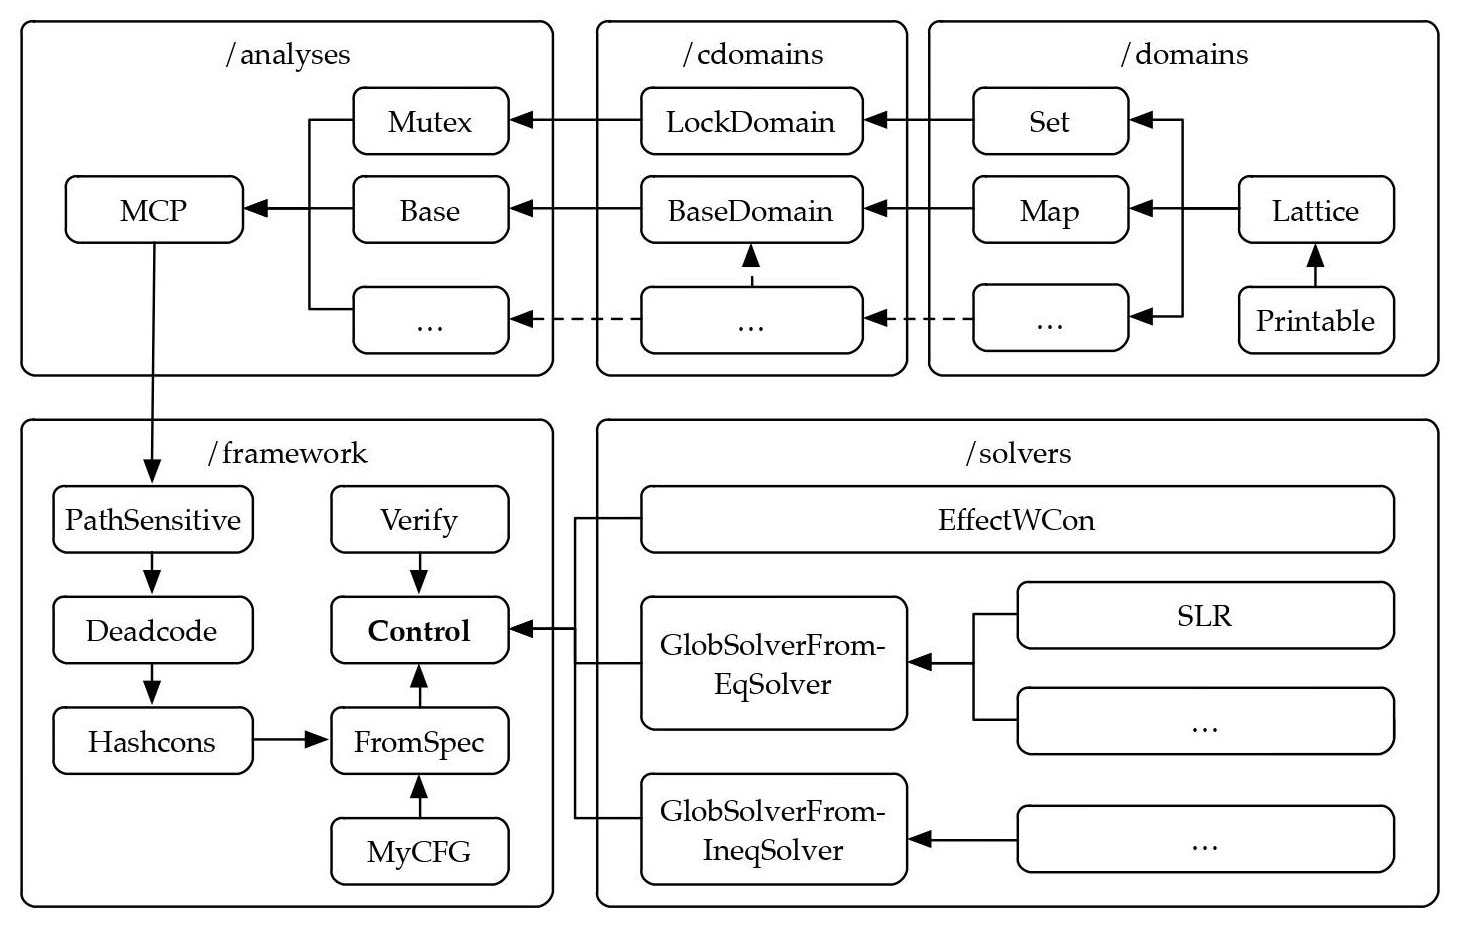
\includegraphics{../figures/goblint_structure_detailed.jpg}
      \caption{Schematic directory structure of \gob. Adapted from \parencite{apinis2014frameworks}}
      \label{fig:gob_structure_detail}
    \end{figure}

    \begin{figure}
      \centering
      \lstinputlisting[language={[Objective]Caml}]{../code/analyses.ml}
      \caption{Simplified Interface for implementing analyses in \gob}
      \label{fig:analysis_interface}
      %TODO: reference github for this file
    \end{figure}

    \begin{figure}
      \centering
      \lstinputlisting[language={[Objective]Caml}]{../code/assign.ml}
      \caption{Implementation of the helper \texttt{taint\_lval} and the \texttt{assign} function}
      \label{fig:assign}
      %TODO: reference github for this file
    \end{figure}



  -- Full New Section: ThreadCreate analysis
